\chapter{Probabilistic Models} \label{chap:models}

\section*{}

\section{Introduction}

Probabilistic or statistical models represent explicit assumptions about a problem domain, in the form of a model. This model usually encompasses random variables, in the form of probability distributions, and the relation and dependence between the variables. \cite{Winn2013}

In the following sections we describe a common way to represent probabilistic models, probabilistic graphical models (PGM) or, simply, graphical models.

\section{Probabilistic Graphical Models}

\begin{figure}[t]
	\begin{center}
		\leavevmode
		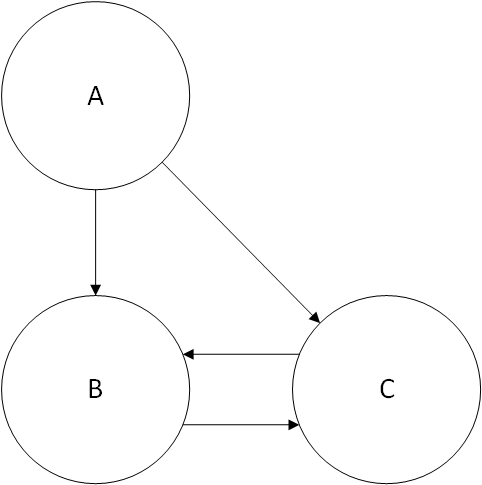
\includegraphics[width=0.36\textwidth]{pgm}
		\caption{Example of a PGM}
		\label{fig:pgm}
	\end{center}
\end{figure}

\ref{fig:pgm}

\section{Bayesian Networks}

\section{Markov Random Fields}

\section{Hidden Markov Models}

\cite{Rabiner1989}

\section{Summary}
